%%%%%%%%%%%%%%%%%%%%%%%%%%%%%%%%%%%%%%%%%%%%%%%%%%%%%%%%%%%%%%%%%%%%%%%%%%%%%%%%%%%%%%%%%%%%%%%%%%%%%%%%%%%%%%%%%%%%%%%%%%%%%%%%%
\chapter{Conclusion}
\label{cha:conclusion}

%%%%%%%%%%%%%%%%%%%%%%%%%%%%%%%%%%%%%%%%%%%%%%%%%%%%%
\section{Results}

\subsection{On the AppStore}

The first release of the application in its revision number 0.9 was uploaded under the name "Hållplats Väst"on the AppStore on March the $8^{th}$ and was ready for sale on March the $13^{th}$. The last version has been renamed "Hållplats SE" as it now covers Göteborg and Stockholm regions.

\begin{figure}[ht]
\center
\subfigure{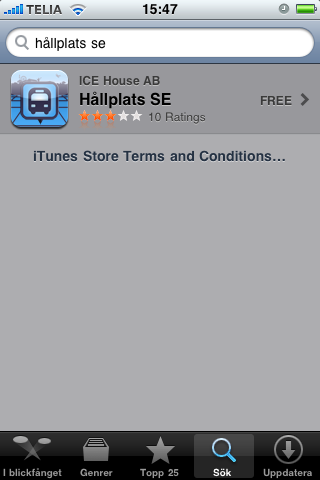
\includegraphics[scale=0.4]{pics/appstore1}}
\hspace{0.3cm}
\subfigure{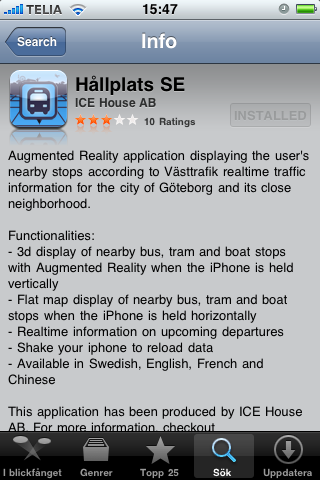
\includegraphics[scale=0.4]{pics/appstore2}}
\caption{Screenshots of the Application on the Appstore}
\label{fig:client_view_hierarchy}
\end{figure}

\subsection{Statistics}
After two months on the store, more than 800 units were downloaded, as shown in Figure \ref{fig:cumulative_downloads}.\\

\begin{figure}[ht]
\center
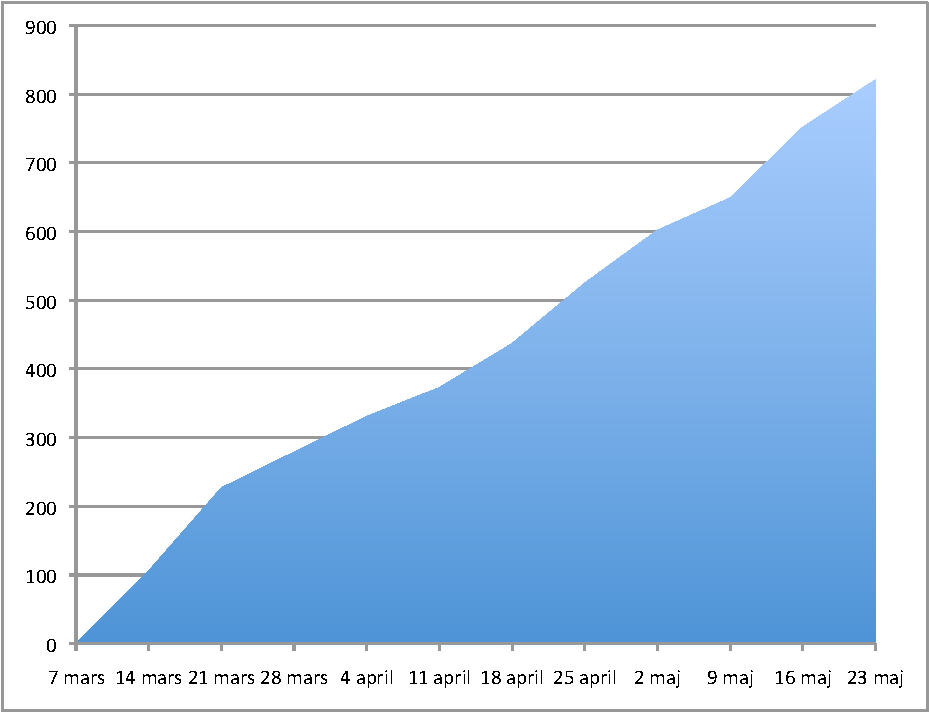
\includegraphics[scale=0.5]{pics/cumulative_downloads}
\caption{Cumulative downloads of the Application on the AppStore}
\label{fig:cumulative_downloads}
\end{figure}

But the number of downloads does not necessary reflects the number of real users of the application, so instead Figure \ref{fig:unique_users} shows the numbers of unique users per day. The average number is around 40 unique users per day, which is rather satisfying.\\

\begin{figure}[ht]
\center
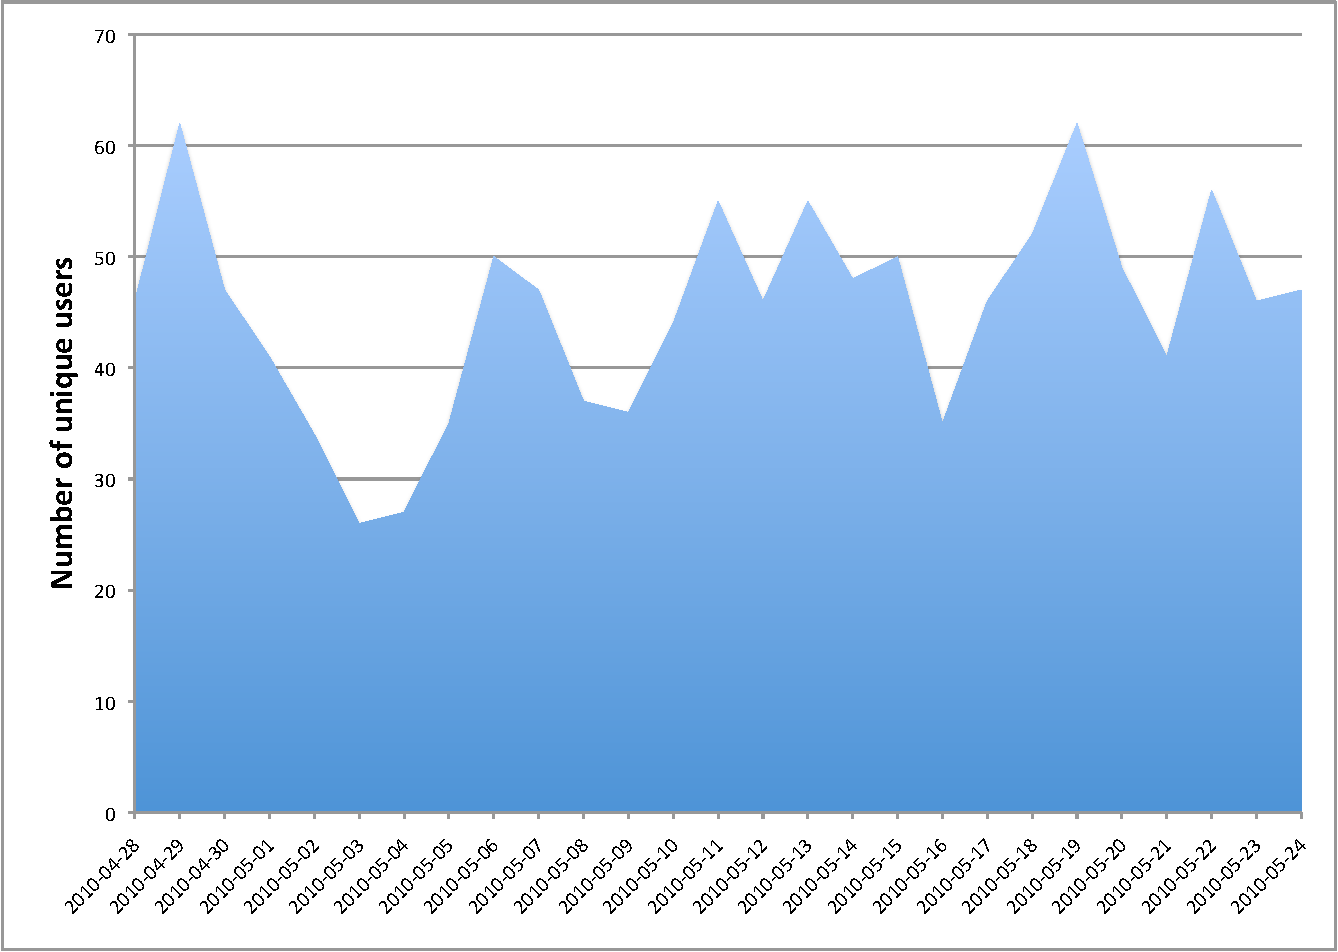
\includegraphics[scale=0.35]{pics/unique_users}
\caption{Unique users per day}
\label{fig:unique_users}
\end{figure}

We can also know the user's location when he uses the application since the URL that is used to request his nearby POI contains his latitude and longitude coordinates. As we can see from Figure \ref{fig:locations_sweden}, users are well spread in the region of Göteborg and Stockholm, even though there is no advertisement made for the last one.\\

\begin{figure}[ht]
\center
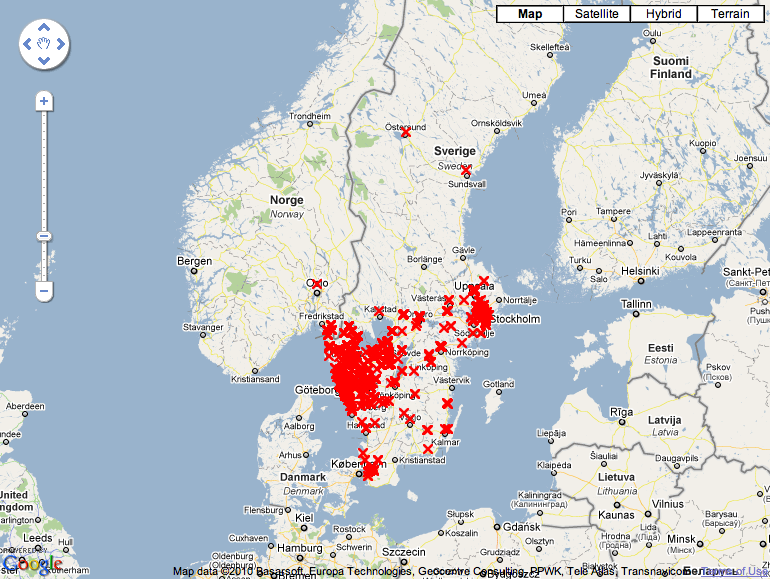
\includegraphics[scale=0.4]{pics/locations_sweden}
\caption{Users' locations in Sweden}
\label{fig:locations_sweden}
\end{figure}

Funny enough to be mentioned, Figure \ref{fig:locations_world} shows that some users also tried the application from Germany, South Korea, China, Singapore, and Qatar.

\begin{figure}[ht]
\center
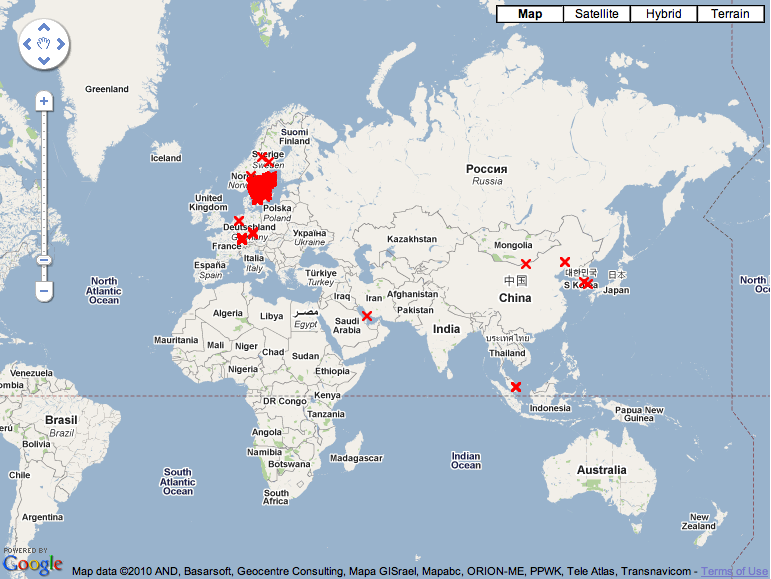
\includegraphics[scale=0.4]{pics/locations_world}
\caption{Users' locations in... the world?}
\label{fig:locations_world}
\end{figure}

\clearpage


%%%%%%%%%%%%%%%%%%%%%%%%%%%%%%%%%%%%%%%%%%%%%%%%%%%%%
\section{Further Considerations}
\subsection{on the Client}

Our implementation of Augmented Reality only relies on GPS, compass and accelerometers inputs to estimate the position of the camera. But an additional input could be the camera itself and the images it captures.\\

Unfortunately, the iPhone SDK does not allow us to access the camera data so for now, but it the camera API will be made public with the release of the iPhone OS4.0 SDK.

\subsection{on the Server}

The server side has been designed in way as to be extensible easily. As such, new cities can be added to the database by creating a Ruby module that talks to the service provider. It would be interesting to extend the availability of the application to all the largest city of Sweden or even Europe, given that the city has a public transport provider with a web service API.

%%%%%%%%%%%%%%%%%%%%%%%%%%%%%%%%%%%%%%%%%%%%%%%%%%%%%
\section{Summary}

We have seen along this paper the implementation of an Augmented Reality for iPhone. The Client side was implemented using Objective-C and the framework necessary for iPhone development. Most of the problem that we faced were concerning trigonometry and projection, plus some restrictions imposed by the SDK that had to be handled.\\

The Server side was implemented using Erlang and Ruby. This part was really interesting and was also the most instructive part of the thesis. It dealt with concurrency, parsing, caching data and much more.\\

More work can be done and the application can be improved in many ways, especially the geographical coverage, but a stable release is already available from the Appstore and more that 800 units have been downloaded since its first release and 40 persons are using each day.\\

